\section{Arquitetura interna}
\label{arquitetura-interna}

O MIST foi desenvolvido para ser utilizado por um administrador do banco de dados que se deseja analisar. O \gls{dba} deve coletar as consultas SQL executadas pela aplicação, o modelo físico do banco de dados e as estatísticas necessárias sobre os dados, convertendo estas informações para arquivos XML utilizados como entrada de dados para a ferramenta, como ilustrado na figura \ref{fig:integracao-solucao}. Como resultado, o ambiente irá apresentar um conjunto de índices recomendados, os quais devem ser avaliados e implementados a critério do \gls{dba}.

\begin{figure}[H]
  \centering
  \caption{Utilização do ambiente desenvolvido.}
  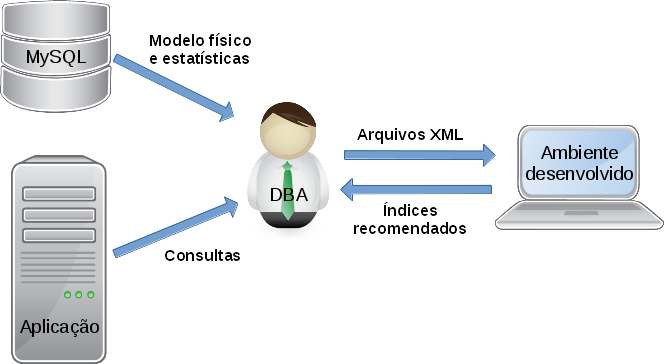
\includegraphics[width=.9\textwidth]{integracao-solucao-tc2.png}
  \fonte{Elaborado pelo autor.}
  \label{fig:integracao-solucao}
\end{figure}

O uso da ferramenta é formado por uma série de operações executadas sequencialmente, conforme apresentado na figura \ref{fig:arquitetura-ambiente}. Na primeira etapa, identificada na figura como (a), é feita a entrada da estrutura das tabelas e as estatísticas dos dados através de um arquivo no formato MSDF (apresentado na seção \ref{formato-msdf}).

\begin{figure}[!ht]
  \centering
  \caption{Arquitetura interna do ambiente desenvolvido.}
  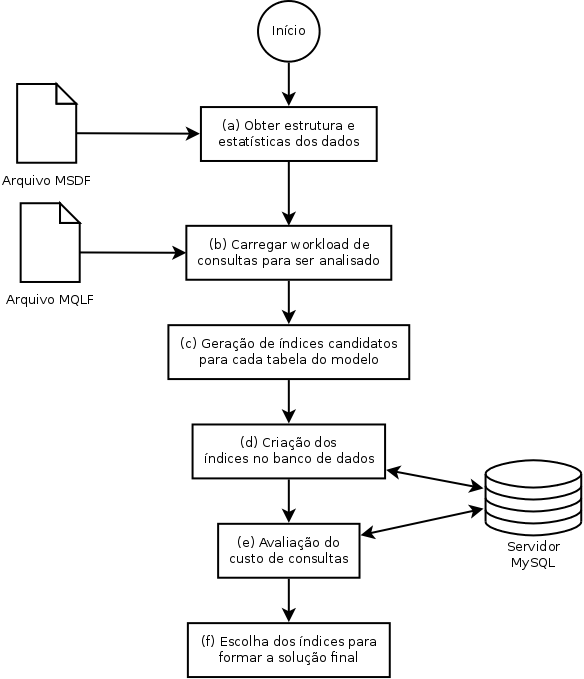
\includegraphics[width=.9\textwidth]{arquitetura-ambiente-tc2.png}
  \fonte{Elaborado pelo autor.}
  \label{fig:arquitetura-ambiente}
\end{figure}

Na etapa (b), o \textit{workload} que deve ser analisado é informado através de um arquivo no formato MQLF, descrito na seção \ref{formato-mqlf}. Em seguida, na fase (c) são gerados os índices candidatos para cada consulta analisada, baseado em boas práticas e recomendações do MySQL. Esta etapa é detalhada na seção \ref{geracao-indices-candidatos}. Posteriormente, em (d) os índices gerados são criados em um banco de dados e o custo das consultas com cada índice é verificado em (e) através de chamadas EXPLAIN para o otimizador do MySQL. Os detalhes destas duas etapas são apresentados na seção \ref{verificacao-custo-indices-candidatos}.

A última etapa (f) da ferramenta consiste em formar o conjunto de índices candidatos que será promovido como recomendação final. Este processo é descrito na seção \ref{geracao-solucao-final}.